\documentclass{ximera}

\title{Practice for Intro to Linear Systems}

%\auor{Matthew Charnley and Jason Nowell}
\usepackage[margin=1.5cm]{geometry}
\usepackage{indentfirst}
\usepackage{sagetex}
\usepackage{lipsum}
\usepackage{amsmath}
\usepackage{mathrsfs}


%%% Random packages added without verifying what they are really doing - just to get initial compile to work.
\usepackage{tcolorbox}
\usepackage{hypcap}
\usepackage{booktabs}%% To get \toprule,\midrule,\bottomrule etc.
\usepackage{nicefrac}
\usepackage{caption}
\usepackage{units}

% This is my modified wrapfig that doesn't use intextsep
\usepackage{mywrapfig}
\usepackage{import}



%%% End to random added packages.


\graphicspath{
    {./figures/}
    {./../figures/}
    {./../../figures/}
}
\renewcommand{\log}{\ln}%%%%
\DeclareMathOperator{\arcsec}{arcsec}
%% New commands


%%%%%%%%%%%%%%%%%%%%
% New Conditionals %
%%%%%%%%%%%%%%%%%%%%


% referencing
\makeatletter
    \DeclareRobustCommand{\myvref}[2]{%
      \leavevmode%
      \begingroup
        \let\T@pageref\@pagerefstar
        \hyperref[{#2}]{%
	  #1~\ref*{#2}%
        }%
        \vpageref[\unskip]{#2}%
      \endgroup
    }%

    \DeclareRobustCommand{\myref}[2]{%
      \leavevmode%
      \begingroup
        \let\T@pageref\@pagerefstar
        \hyperref[{#2}]{%
	  #1~\ref*{#2}%
        }%
      \endgroup
    }%
\makeatother

\newcommand{\figurevref}[1]{\myvref{Figure}{#1}}
\newcommand{\figureref}[1]{\myref{Figure}{#1}}
\newcommand{\tablevref}[1]{\myvref{Table}{#1}}
\newcommand{\tableref}[1]{\myref{Table}{#1}}
\newcommand{\chapterref}[1]{\myref{chapter}{#1}}
\newcommand{\Chapterref}[1]{\myref{Chapter}{#1}}
\newcommand{\appendixref}[1]{\myref{appendix}{#1}}
\newcommand{\Appendixref}[1]{\myref{Appendix}{#1}}
\newcommand{\sectionref}[1]{\myref{\S}{#1}}
\newcommand{\subsectionref}[1]{\myref{subsection}{#1}}
\newcommand{\subsectionvref}[1]{\myvref{subsection}{#1}}
\newcommand{\exercisevref}[1]{\myvref{Exercise}{#1}}
\newcommand{\exerciseref}[1]{\myref{Exercise}{#1}}
\newcommand{\examplevref}[1]{\myvref{Example}{#1}}
\newcommand{\exampleref}[1]{\myref{Example}{#1}}
\newcommand{\thmvref}[1]{\myvref{Theorem}{#1}}
\newcommand{\thmref}[1]{\myref{Theorem}{#1}}


\renewcommand{\exampleref}[1]{ {\color{red} \bfseries Normally a reference to a previous example goes here.}}
\renewcommand{\figurevref}[1]{ {\color{red} \bfseries Normally a reference to a previous figure goes here.}}
\renewcommand{\tablevref}[1]{ {\color{red} \bfseries Normally a reference to a previous table goes here.}}
\renewcommand{\Appendixref}[1]{ {\color{red} \bfseries Normally a reference to an Appendix goes here.}}
\renewcommand{\exercisevref}[1]{ {\color{red} \bfseries Normally a reference to a previous exercise goes here.}}



\newcommand{\R}{\mathbb{R}}

%% Example Solution Env.
\def\beginSolclaim{\par\addvspace{\medskipamount}\noindent\hbox{\bf Solution:}\hspace{0.5em}\ignorespaces}
\def\endSolclaim{\par\addvspace{-1em}\hfill\rule{1em}{0.4pt}\hspace{-0.4pt}\rule{0.4pt}{1em}\par\addvspace{\medskipamount}}
\newenvironment{exampleSol}[1][]{\beginSolclaim}{\endSolclaim}

%% General figure formating from original book.
\newcommand{\mybeginframe}{%
\begin{tcolorbox}[colback=white,colframe=lightgray,left=5pt,right=5pt]%
}
\newcommand{\myendframe}{%
\end{tcolorbox}%
}

%%% Eventually return and fix this to make matlab code work correctly.
%% Define the matlab environment as another code environment
%\newenvironment{matlab}
%{% Begin Environment Code
%{ \centering \bfseries Matlab Code }
%\begin{code}
%}% End of Begin Environment Code
%{% Start of End Environment Code
%\end{code}
%}% End of End Environment Code


% this one should have a caption, first argument is the size
\newenvironment{mywrapfig}[2][]{
 \wrapfigure[#1]{r}{#2}
 \mybeginframe
 \centering
}{%
 \myendframe
 \endwrapfigure
}

% this one has no caption, first argument is size,
% the second argument is a larger size used for HTML (ignored by latex)
\newenvironment{mywrapfigsimp}[3][]{%
 \wrapfigure[#1]{r}{#2}%
 \centering%
}{%
 \endwrapfigure%
}
\newenvironment{myfig}
    {%
    \begin{figure}[h!t]
        \mybeginframe%
        \centering%
    }
    {%
        \myendframe
    \end{figure}%
    }


% graphics include
\newcommand{\diffyincludegraphics}[3]{\includegraphics[#1]{#3}}
\newcommand{\myincludegraphics}[3]{\includegraphics[#1]{#3}}
\newcommand{\inputpdft}[1]{\subimport*{../figures/}{#1.pdf_t}}


%% Not sure what these even do? They don't seem to actually work... fun!
%\newcommand{\mybxbg}[1]{\tcboxmath[colback=white,colframe=black,boxrule=0.5pt,top=1.5pt,bottom=1.5pt]{#1}}
%\newcommand{\mybxsm}[1]{\tcboxmath[colback=white,colframe=black,boxrule=0.5pt,left=0pt,right=0pt,top=0pt,bottom=0pt]{#1}}
\newcommand{\mybxsm}[1]{#1}
\newcommand{\mybxbg}[1]{#1}

%%% Something about tasks for practice/hw?
\usepackage{tasks}
\usepackage{footnote}
\makesavenoteenv{tasks}


%% For pdf only?
\newcommand{\diffypdfversion}[1]{#1}


%% Kill ``cite'' and go back later to fix it.
\renewcommand{\cite}[1]{}


%% Currently we can't really use index or its derivatives. So we are gonna kill them off.
\renewcommand{\index}[1]{}
\newcommand{\myindex}[1]{#1}







\begin{document}
\begin{abstract}
Why?
\end{abstract}
\maketitle


\begin{exercise}
    Does $x_1(t) = 2e^{-t} - 2e^{-2t}$, $x_2(t) = e^{-t} - 2e^{-2t}$ solve the system $x_1' = - 2x_2 $, $x_2' = x_1 - 3x_2$?
    \begin{multipleChoice}
        \choice[correct]{Yes.}
        \choice{No.}
    \end{multipleChoice}
\end{exercise}
%\comboSol
%{%
%It works
%}

\begin{exercise}
    Does that $x_1(t) = -2te^{-3t} - 2e^{-3t}$, $x_2(t) = 2te^{-3t} + 3e^{-3t}$ solve the system $x_1' = -5x_1 - 2x_2 $, $x_2' = 2x_1 - x_2$?
    \begin{multipleChoice}
        \choice[correct]{Yes.}
        \choice{No.}
    \end{multipleChoice}
\end{exercise}
%\comboSol
%{%
%It works
%}

\begin{exercise}
    Find the general solution of $x_1' = x_2 - x_1 + t$, $x_2' = x_2$. [Use $A$ and $B$ for your arbitrary constants] \\
    $x_1 = \answer{\frac{A}{2}e^t + (t-1) + Be^{-t}}$, $x_2 = \answer{Ae^t}$
\end{exercise}
%\comboSol
%{%
%$x_1 = \frac{C_1}{2}e^t + (t-1) + C_2e^{-t}$, $x_2 = C_1e^t$
%}

\begin{exercise}
    Find the general solution of $x_1' = 3 x_1 - x_2 + e^t$, $x_2' = x_1$. [Use $A$. $B$ and $C$ for your arbitrary constants] \\
    $x_1 = \answer{\frac{3+\sqrt{5}}{2}Ae^{\frac{3+\sqrt{5}}{2}t} + \frac{3-\sqrt{5}}{2}Be^{\frac{3-\sqrt{5}}{2}t} - \frac{1}{2}Ce^t}$, $x_2 = \answer{Ae^{\frac{3+\sqrt{5}}{2}t} + Be^{\frac{3-\sqrt{5}}{2}t} - \frac{1}{2}Ce^t}$
\end{exercise}
%\comboSol
%{%
%$x_1 = \frac{3+\sqrt{5}}{2}C_1e^{\frac{3+\sqrt{5}}{2}t} + \frac{3-\sqrt{5}}{2}C_2e^{\frac{3-\sqrt{5}}{2}t} - \frac{1}{2}Ae^t$, $x_2 = C_1e^{\frac{3+\sqrt{5}}{2}t} + C_2e^{\frac{3-\sqrt{5}}{2}t} - \frac{1}{2}Ae^t$
%}

\begin{exercise}%
    Find the general solution to $y_1' = 3 y_1$, $y_2' = y_1 + y_2$, $y_3' = y_1 + y_3$. [Use $A$. $B$ and $C$ for your arbitrary constants]\\
    $y_1 = \answer{A e^{3x}}$,\\
    $y_2 = y(x) = \answer{B e^x+ \frac{A}{2} e^{3 x}}$,\\
    $y_3 = y(x) = \answer{C e^x+ \frac{A}{2} e^{3 x}}$
\end{exercise}
%\exsol{%
%$y_1 = C_1 e^{3x}$,
%$y_2 = y(x) = C_2 e^x+ \frac{C_1}{2} e^{3 x}$,
%$y_3 = y(x) = C_3 e^x+ \frac{C_1}{2} e^{3 x}$
%}

\begin{exercise}%
    Solve $y'=2x$, $x'=x+y$, $x(0)=1$, $y(0)=3$.\\
    $x = \answer{\frac{5}{3} e^{2t} - \frac{2}{3} e^{-t}}$,\\
    $y = \answer{\frac{5}{3} e^{2t} + \frac{4}{3} e^{-t}}$
\end{exercise}
%\exsol{%
%$x=\frac{5}{3} e^{2t} - \frac{2}{3} e^{-t}$,
%$y=\frac{5}{3} e^{2t} + \frac{4}{3} e^{-t}$
%}


\begin{exercise}
    Write $ay'' + by' + cy = f(x)$ as a first order system of ODEs.\\
    $\vec{x} ' = \left[\begin{smallmatrix} \answer{0} & \answer{1} \\ -\frac{c}{a} & \answer{-\frac{b}{a}} \end{smallmatrix}\right] \vec{x} + \left[\begin{smallmatrix}  \answer{0} \\ \answer{\frac{1}{a}}f(x) \end{smallmatrix}\right]$
\end{exercise}
%\comboSol
%{%
%$\vec{x}\ ' = \left[\begin{smallmatrix} 0 & 1 \\ -\frac{c}{a} & -\frac{b}{a} \end{smallmatrix}\right] \vec{x} + \left[\begin{smallmatrix}  0 \\ \frac{1}{a}f(x) \end{smallmatrix}\right]$
%}

\begin{exercise}
    Write $x'' + y^2 y' - x^3 = \sin(t)$, $y'' + {(x'+y')}^2 -x = 0$ as a first order system of ODEs.\\
    %$\left[\begin{smallmatrix} u_1 \\ u_2 \\ u_3 \\ u_4 \end{smallmatrix}\right]' = \left[\begin{smallmatrix} u_2 \\ \sin(t) + u_1^3 - u_3^2u_4 \\ u_4 \\ u_1 - (u_3 + u_4)^2 \end{smallmatrix}\right]$
\end{exercise}
%\comboSol
%{%
%$\left[\begin{smallmatrix} u_1 \\ u_2 \\ u_3 \\ u_4 \end{smallmatrix}\right]' = \left[\begin{smallmatrix} u_2 \\ \sin(t) + u_1^3 - u_3^2u_4 \\ u_4 \\ u_1 - (u_3 + u_4)^2 \end{smallmatrix}\right]$
%}

\begin{exercise}%
    Write $x''' = x + t$ as a first order system.
\end{exercise}
%\exsol{%
%$x_1' = x_2$,
%$x_2' = x_3$,
%$x_3' = x_1+t$
%}

\begin{exercise}%
    Write $y_1'' + y_1 + y_2 = t$, $y_2'' + y_1 - y_2 = t^2$ as a first order system.
\end{exercise}
%\exsol{%
%$y_3' + y_1 + y_2 = t$, 
%$y_4' + y_1 - y_2 = t^2$,
%$y_1' = y_3$,
%$y_2' = y_4$
%}

\begin{exercise}
    Write $y^{(4)} - t^2 y''' + e^t y' - (2t+1)y = \cos(t)$ as a first order system.\\
    $\vec{u}' = \left[\begin{smallmatrix}  \answer{0} & \answer{1} & 0 & 0 \\ \answer{0} & 0 & \answer{1} & \answer{0} \\ 0 & \answer{0} & \answer{0} & 1 \\ \answer{2t+1} & -e^t & \answer{0} & t^2 \end{smallmatrix}\right]\vec{u} + \left[\begin{smallmatrix} 0 \\ 0 \\ 0 \\ \cos(t) \end{smallmatrix}\right]$
\end{exercise}
%\comboSol
%{%
%$\vec{u}' = \left[\begin{smallmatrix}  0 & 1 & 0 & 0 \\ 0 & 0 & 1 & 0 \\ 0 & 0 & 0 & 1 \\ 2t+1 & -e^t & 0 & t^2 \end{smallmatrix}\right]\vec{u} + \left[\begin{smallmatrix} 0 \\ 0 \\ 0 \\ \cos(t) \end{smallmatrix}\right]$
%}

\begin{exercise}
    Write the initial value problem 
    \[ 
        y'' - 2xy' + 3y = \sin(x) \qquad y(0) = 1,\ y'(0) = -2 
    \] 
    as an initial value problem for a first order system of ODEs. Make sure to indicate how the initial condition appears as a part of this problem. \\
    $\vec{u}' = \left[\begin{smallmatrix}  0 & \answer{1} \\ -3 & \answer{2x} \end{smallmatrix}\right]\vec{x} + \left[\begin{smallmatrix}  \answer{0} \\ \sin(x) \end{smallmatrix}\right]$, $\vec{u}(0) = \left[\begin{smallmatrix}  \answer{1} \\ -2 \end{smallmatrix}\right]$
\end{exercise}
%\comboSol
%{%
%$\vec{u}' = \left[\begin{smallmatrix}  0 & 1 \\ -3 & 2x \end{smallmatrix}\right]\vec{x} + \left[\begin{smallmatrix}  0 \\ \sin(x) \end{smallmatrix}\right]$, $\vec{u}(0) = \left[\begin{smallmatrix}  1 \\ -2 \end{smallmatrix}\right]$
%}

\begin{exercise}
    Write the initial value problem 
    \[ 
        y'' - (y+1)^2 y' - e^{xy} = \cos(x) \qquad y(0) = -1,\ y'(0) = 5 
    \] 
    as an initial value problem for a first order system of ODEs. Make sure to indicate how the initial condition appears as a part of this problem.\\
    $\vec{u}' = \left[\begin{smallmatrix}  u_2 \\ \cos(x) + e^{xu_1} + (u_1 + 1)^2u_2 \end{smallmatrix}\right]$, $\vec{u}(0) = \left[\begin{smallmatrix}  \answer{-1} \\ \answer{5} \end{smallmatrix}\right]$
    \begin{problem}
        Can this be written in matrix form? %Why or why not?
        \begin{multipleChoice}
            \choice{Yes.}
            \choice[correct]{No.}
        \end{multipleChoice}
    \end{problem}
\end{exercise}
%\comboSol
%{%
%$\vec{u}' = \left[\begin{smallmatrix}  u_2 \\ \cos(x) + e^{xu_1} + (u_1 + 1)^2u_2 \end{smallmatrix}\right]$, $\vec{u}(0) = \left[\begin{smallmatrix}  -1 \\ 5 \end{smallmatrix}\right]$. Non-linear.
%}

\begin{exercise}
    Write the initial value problem 
    \[ 
        y^{(4)} + e^x y'' - 4\cos(x)y' + (x^2 + 1)y = \frac{1}{x-3} \qquad y(0) = 2,\ y'(0) = -3,\ y''(0) = 0,\ y^{(3)}(0) = 1 
    \] 
    as an initial value problem for a first order system of ODEs. Make sure to indicate how the initial condition appears as a part of this problem. \\
    $\vec{u}' = \left[\begin{smallmatrix}  \answer{0} & 1 & \answer{0} & 0 \\ \answer{0} & \answer{0} & 1 & \answer{0} \\ \answer{0} & 0 & \answer{0} & \answer{1} \\ \answer{-(x^2 + 1)} & \answer{4\cos(x)} & -e^x & \answer{0} \end{smallmatrix}\right] \vec{u} + \left[\begin{smallmatrix} \answer{0} \\ 0 \\ \answer{0} \\ \answer{\frac{1}{x-3}} \end{smallmatrix}\right]$, $\vec{u}(0) = \left[\begin{smallmatrix} \answer{-2} \\ \answer{-3} \\ 0 \\ \answer{1} \end{smallmatrix}\right]$
\end{exercise}
%\comboSol
%{%
%$\vec{u}' = \left[\begin{smallmatrix}  0 & 1 & 0 & 0 \\ 0 & 0 & 1 & 0 \\ 0 & 0 & 0 & 1 \\ -(x^2 + 1) & 4\cos(x) & -e^x & 0 \end{smallmatrix}\right] \vec{u} + \left[\begin{smallmatrix} 0 \\ 0 \\ 0 \\ \frac{1}{x-3} \end{smallmatrix}\right]$, $\vec{u}(0) = \left[\begin{smallmatrix} -2 \\ -3 \\ 0 \\ 1 \end{smallmatrix}\right]$.
%}

\begin{exercise}
    Suppose two masses on carts on frictionless surface are at displacements $x_1$ and $x_2$ as in example \ref{sintro:carts-example}. Suppose that a rocket applies force $F$ in the positive direction on cart $x_1$.  Set up the system of equations.\\
    $mx_1'' = \answer{k(x_2 - x_1)} + F$,  $mx_2'' = \answer{-k}(x_2 - x_1)$
\end{exercise}
%\comboSol
%{%
%$mx_1'' = k(x_2 - x_1) + F,\ mx_2''  =-k(x_2 - x_1)$
%}

\begin{exercise}%
    Suppose two masses on carts on frictionless surface are at  displacements $x_1$ and $x_2$ as in example \ref{sintro:carts-example}. Suppose initial displacement is $x_1(0)=x_2(0)=0$, and initial velocity is $x_1'(0) = x_2'(0) = a$ for some number $a$. Use your intuition to solve the system, explain your reasoning. $x_1 = x_2 = \answer{at}$
\end{exercise}
%\exsol{%
%$x_1 = x_2 = at$.  Explanation of the intuition is left to reader.
%}

\begin{exercise}
    Suppose the tanks are as in example \ref{sintro:closedbrine-example}, starting both at volume $V$, but now the rate of flow from tank 1 to tank 2 is $r_1$, and rate of flow from tank 2 to tank 1 is $r_2$.  In particular, the volumes will now be changing.  Set up the system of equations.\\
    $V_1(t) = V + (r_2 - r_1)\answer{t}$, $V_2(t) = V + (r_1 - r_2)\answer{t}$ \\
    $\frac{dx_1}{dt} = r_2\left(\frac{x_2}{\answer{V} + (r_1 - r_2)\answer{t}}\right)  - r_1\left(\frac{x_1}{\answer{V} + (r_2 - r_1)\answer{t}}\right)$ \quad
    $\frac{dx_2}{dt} = \answer{r_1\left(\frac{x_1}{V + (r_2 - r_1)t}\right) - r_2\left(\frac{x_2}{V + (r_1 - r_2)t}\right)}$ \\
\end{exercise}
%\comboSol
%{%
%$V_1(t) = V + (r_2 - r_1)t$, $V_2(t) = V + (r_1 - r_2)t$ \\
%$\frac{dx_1}{dt} = r_2\left(\frac{x_2}{V + (r_1 - r_2)t}\right)  - r_1\left(\frac{x_1}{V + (r_2 - r_1)t}\right)$ \quad
%$\frac{dx_2}{dt} = r_1\left(\frac{x_1}{V + (r_2 - r_1)t}\right)  - r_2\left(\frac{x_2}{V + (r_1 - r_2)t}\right)$ \\
%}

\begin{exercise}%
    Suppose the tanks are as in example \ref{sintro:closedbrine-example} except that clean water flows in at the rate $s$ liters per second into tank 1, and brine flows out of tank 2 and into the sewer also at the rate of $s$ liters per second. We also adjust the flow rate of the line from tank 1 to tank 2 to be $r+s$ liters per second.
    \begin{itemize}
        \item Draw the picture.
        \item Set up the system of equations.\\
            $x_1' = \answer{\frac{r}{V} (x_2-x_1)}$,\\
            $x_2' = \answer{\frac{r}{V} x_1- \frac{r-s}{V}x_2}$.
        \item Intuitively, what happens as $t$ goes to infinity, explain.\\
            As $t$ goes to infinity, both $x_1$ and $x_2$ go to $\answer{0}$
    \end{itemize}
\end{exercise}
%\exsol{%
%a) Left to reader.
%\quad b) 
%$x_1' = \frac{r}{V} (x_2-x_1)$,
%$x_2' = \frac{r}{V} x_1- \frac{r-s}{V}x_2$.
%\quad c) As $t$ goes to infinity, both $x_1$ and $x_2$ go to zero,
%explanation is left to reader.
%}

\begin{exercise}%
    Match the systems of differential equations below to their corresponding slope fields. Justify.
    \begin{equation*}
        (i)\ 
        \begin{cases} 
            \frac{dx}{dt} &= x+y \\ 
            \frac{dy}{dt} &= 2y-x 
        \end{cases} 
        \qquad (ii)\ 
        \begin{cases} 
            \frac{dx}{dt} &= x-y \\ 
            \frac{dy}{dt} &= x^2 + y 
        \end{cases} 
        \qquad (iii)\ 
        \begin{cases} 
            \frac{dx}{dt} &= x^2 - y^2 \\ 
            \frac{dy}{dt} &= 3x-1 
        \end{cases}
    \end{equation*}
    \begin{itemize}
        \item \parbox[c]{2in}{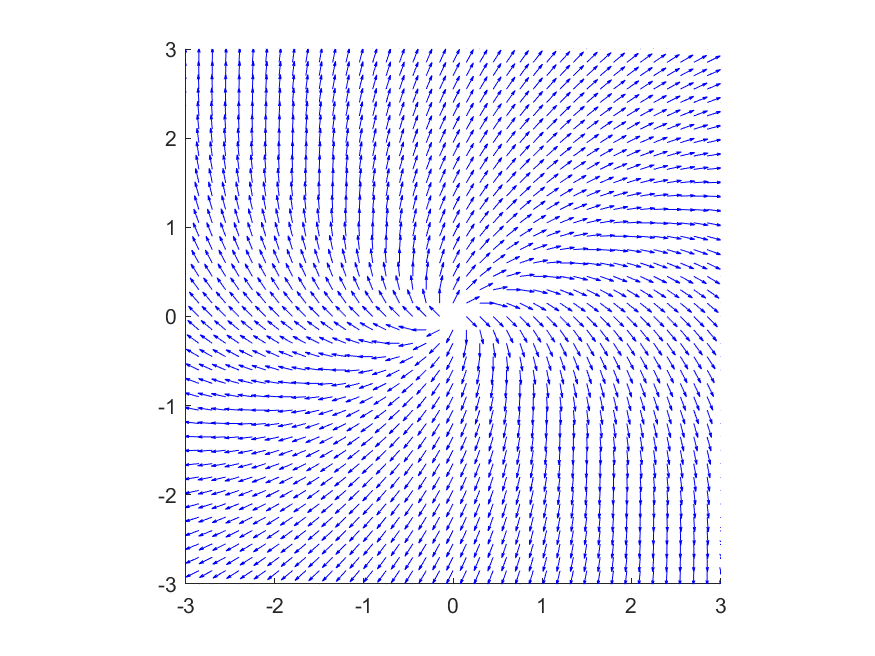
\includegraphics[width=1.75in]{sysslopeEx1_1}}
            \begin{multipleChoice}
                \choice[correct]{i}
                \choice{ii}
                \choice{iii}
            \end{multipleChoice}
        \item \parbox[c]{2in}{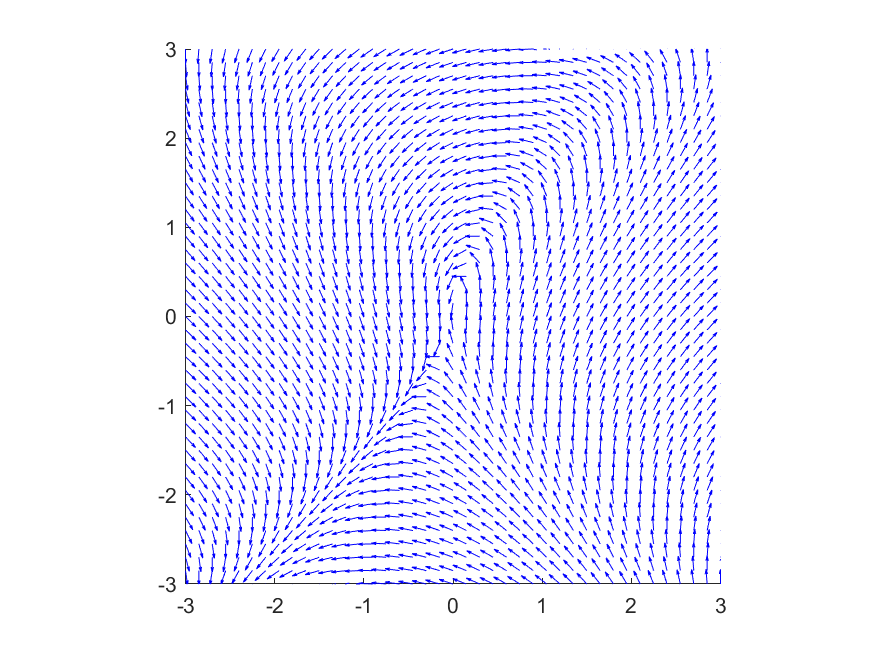
\includegraphics[width=1.75in]{sysslopeEx1_3}}
            \begin{multipleChoice}
                \choice{i}
                \choice{ii}
                \choice[correct]{iii}
            \end{multipleChoice}
        \item \parbox[c]{2in}{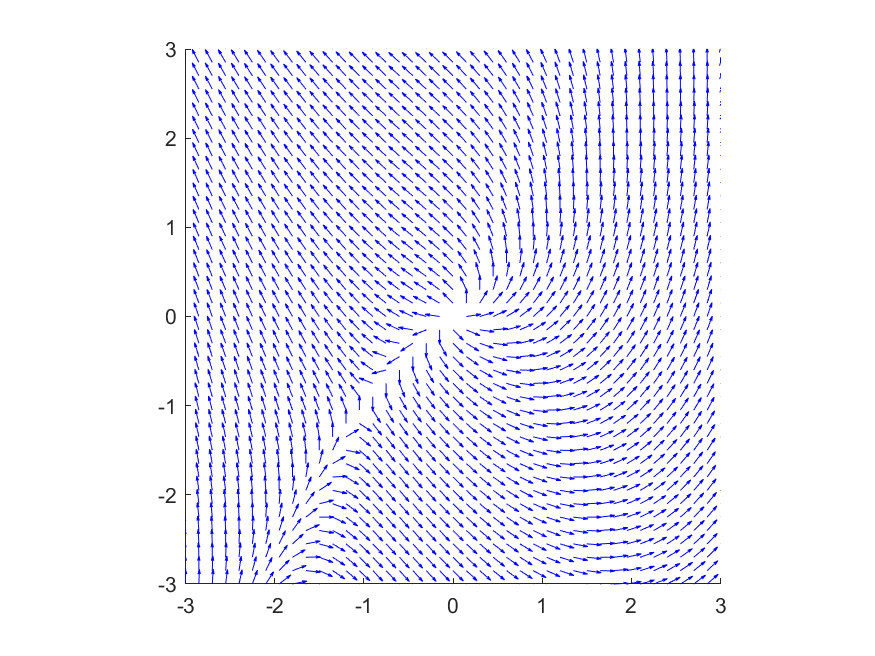
\includegraphics[width=1.75in]{sysslopeEx1_2}}
            \begin{multipleChoice}
                \choice{i}
                \choice[correct]{ii}
                \choice{iii}
            \end{multipleChoice}
    \end{itemize}
\end{exercise}
%\exsol{%
%a) (i), \quad
%b) (iii), \quad
%c) (ii) \quad
%Justification left to reader.
%}

\begin{exercise}
    Match the systems of differential equations below to their corresponding slope fields. Justify.
    \begin{equation*}
        (i)\ 
        \begin{cases} 
            \frac{dx}{dt} &= 2x+y \\ 
            \frac{dy}{dt} &= y - x^2 
        \end{cases} 
        \qquad (ii)\ 
        \begin{cases} 
            \frac{dx}{dt} &= x^2 \\ 
            \frac{dy}{dt} &= x-y 
        \end{cases} 
        \qquad (iii)\ 
        \begin{cases} 
            \frac{dx}{dt} &= y+2 \\ 
            \frac{dy}{dt} &= x+y+1 
        \end{cases}
    \end{equation*}
    \begin{itemize}
        \item \parbox[c]{2in}{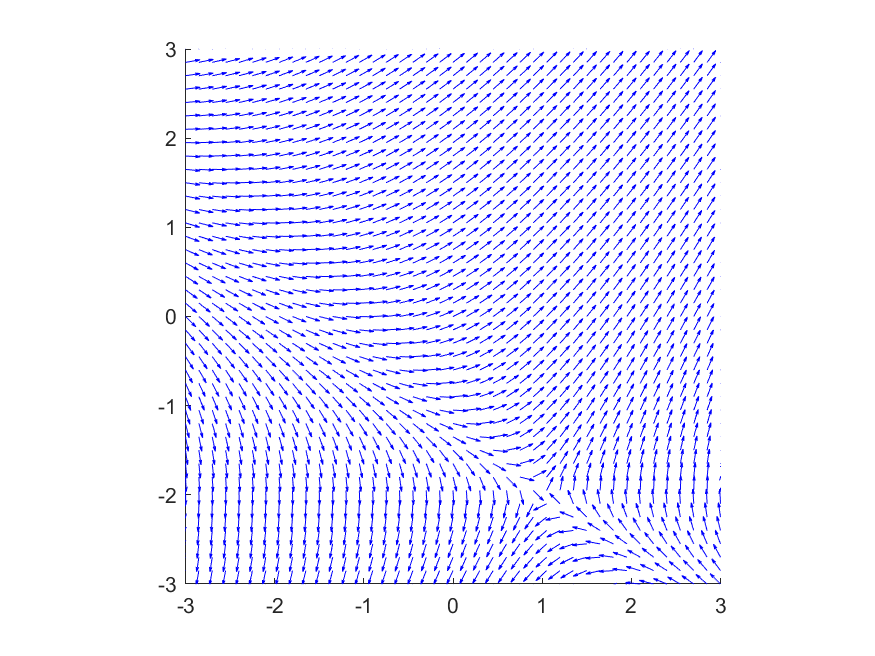
\includegraphics[width=1.75in]{sysslopeEx2_3}}
            \begin{multipleChoice}
                \choice{i}
                \choice{ii}
                \choice[correct]{iii}
            \end{multipleChoice}
        \item \parbox[c]{2in}{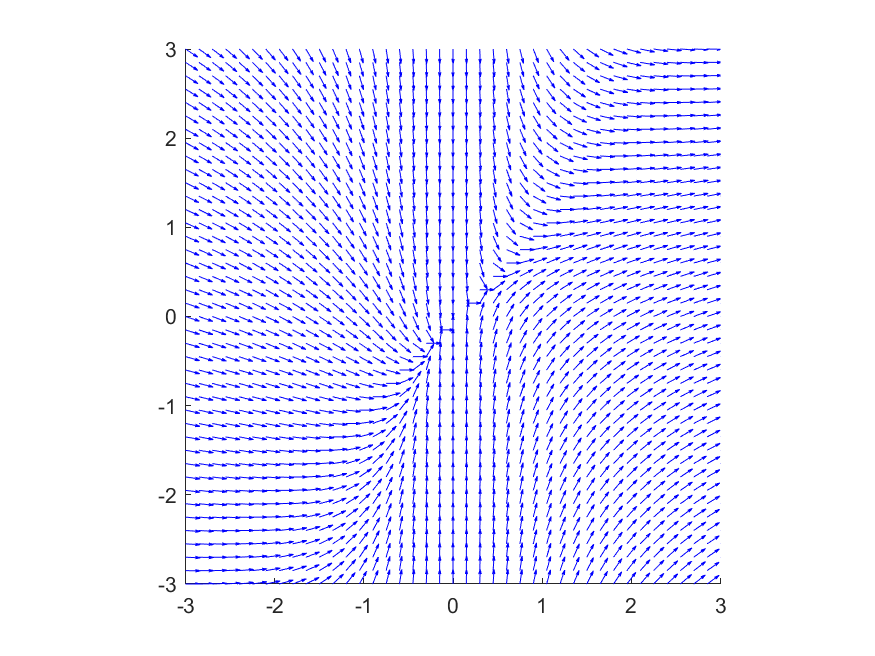
\includegraphics[width=1.75in]{sysslopeEx2_2}}
            \begin{multipleChoice}
                \choice{i}
                \choice[correct]{ii}
                \choice{iii}
            \end{multipleChoice}
        \item \parbox[c]{2in}{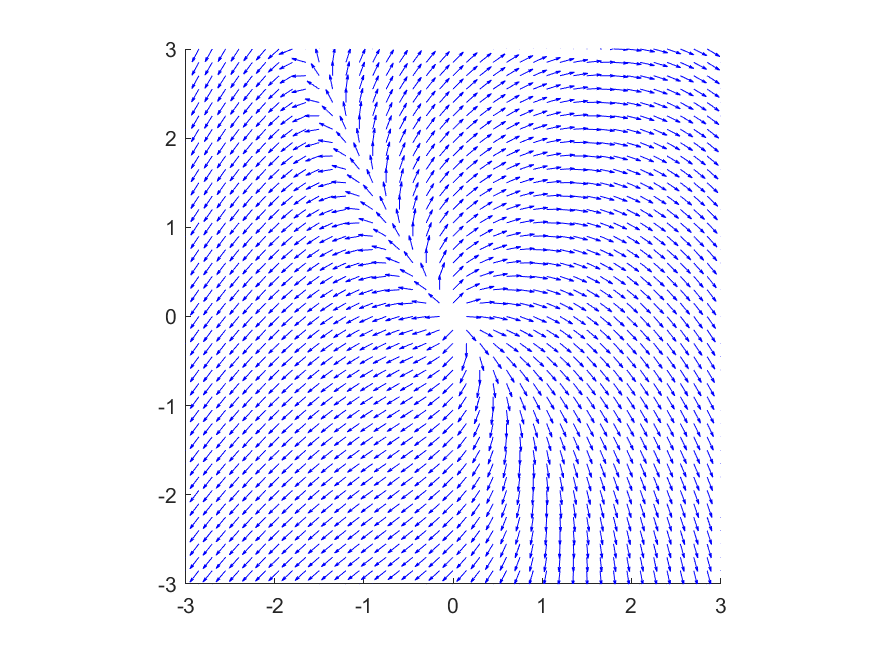
\includegraphics[width=1.75in]{sysslopeEx2_1}}
            \begin{multipleChoice}
                \choice[correct]{i}
                \choice{ii}
                \choice{iii}
            \end{multipleChoice}
    \end{itemize}
\end{exercise}
%\exsol{%
%a) (iii), \quad
%b) (ii), \quad
%c) (i) \quad
%Justification left to reader.
%}


\end{document}